% Created by tikzDevice version 0.12.3.1 on 2022-09-02 13:47:07
% !TEX encoding = UTF-8 Unicode
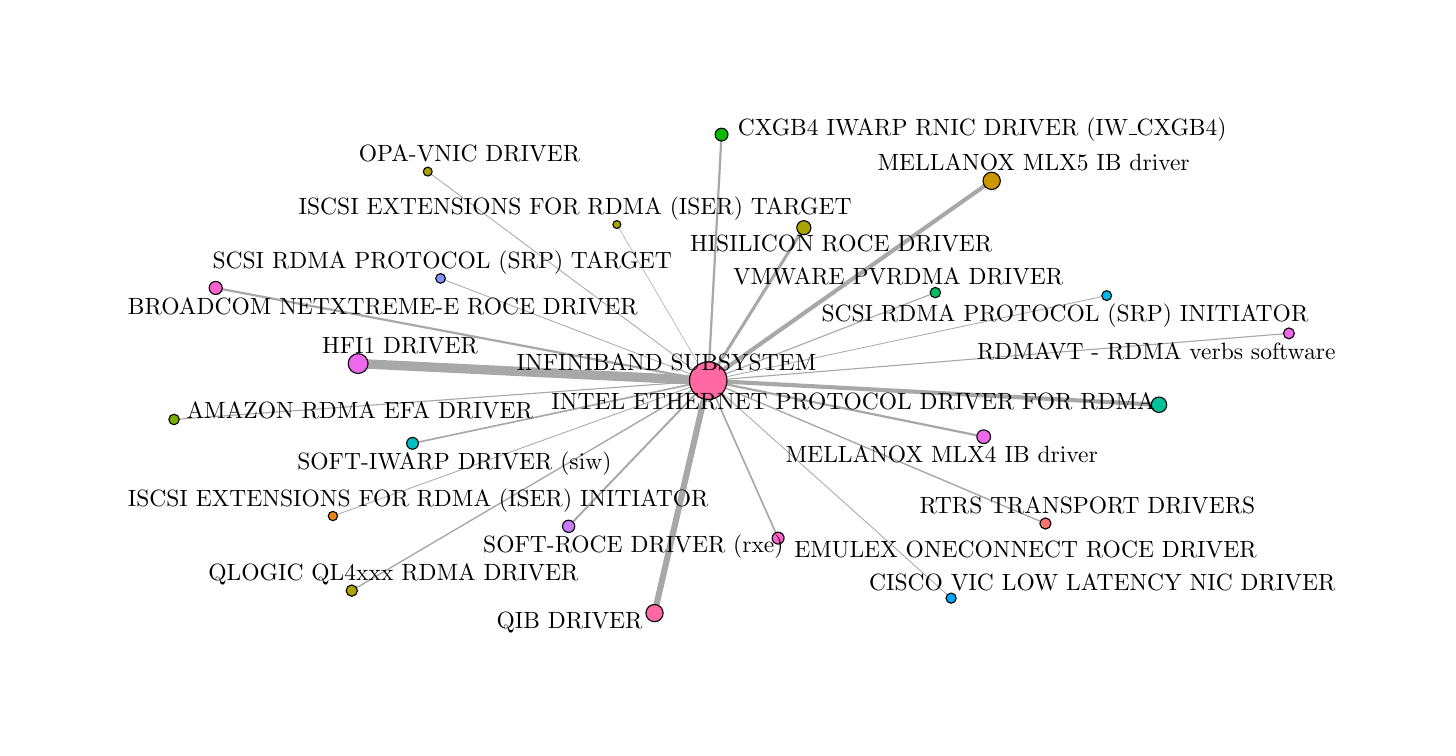
\begin{tikzpicture}[x=1pt,y=1pt]
\definecolor{fillColor}{RGB}{255,255,255}
\path[use as bounding box,fill=fillColor,fill opacity=0.00] (0,0) rectangle (505.89,252.94);
\begin{scope}
\path[clip] (  0.00,  0.00) rectangle (505.89,252.94);
\definecolor{fillColor}{RGB}{255,255,255}

\path[fill=fillColor] (  0.00,  0.00) rectangle (505.89,252.94);
\end{scope}
\begin{scope}
\path[clip] ( 32.75, 32.75) rectangle (475.89,222.94);
\definecolor{drawColor}{gray}{0.66}

\path[draw=drawColor,line width= 0.4pt,line join=round] ( 52.89,111.36) -- (245.91,125.38);

\path[draw=drawColor,line width= 0.8pt,line join=round] ( 67.94,158.89) -- (245.91,125.38);

\path[draw=drawColor,line width= 0.3pt,line join=round] (333.68, 46.80) -- (245.91,125.38);

\path[draw=drawColor,line width= 0.8pt,line join=round] (250.73,214.30) -- (245.91,125.38);

\path[draw=drawColor,line width= 0.6pt,line join=round] (271.17, 68.49) -- (245.91,125.38);

\path[draw=drawColor,line width= 3.4pt,line join=round] (119.41,131.56) -- (245.91,125.38);

\path[draw=drawColor,line width= 1.1pt,line join=round] (280.46,180.65) -- (245.91,125.38);

\path[draw=drawColor,line width= 1.5pt,line join=round] (245.91,125.38) -- (408.80,116.68);

\path[draw=drawColor,line width= 0.3pt,line join=round] (245.91,125.38) -- (110.29, 76.47);

\path[draw=drawColor,line width= 0.2pt,line join=round] (245.91,125.38) -- (212.90,181.79);

\path[draw=drawColor,line width= 0.8pt,line join=round] (245.91,125.38) -- (345.46,105.13);

\path[draw=drawColor,line width= 1.5pt,line join=round] (245.91,125.38) -- (348.33,197.58);

\path[draw=drawColor,line width= 0.3pt,line join=round] (245.91,125.38) -- (144.57,200.93);

\path[draw=drawColor,line width= 2.2pt,line join=round] (245.91,125.38) -- (226.51, 41.40);

\path[draw=drawColor,line width= 0.5pt,line join=round] (245.91,125.38) -- (117.11, 49.52);

\path[draw=drawColor,line width= 0.4pt,line join=round] (245.91,125.38) -- (455.75,142.47);

\path[draw=drawColor,line width= 0.5pt,line join=round] (245.91,125.38) -- (367.76, 73.78);

\path[draw=drawColor,line width= 0.3pt,line join=round] (245.91,125.38) -- (389.90,156.12);

\path[draw=drawColor,line width= 0.3pt,line join=round] (245.91,125.38) -- (149.19,162.33);

\path[draw=drawColor,line width= 0.6pt,line join=round] (245.91,125.38) -- (139.07,102.73);

\path[draw=drawColor,line width= 0.7pt,line join=round] (245.91,125.38) -- (195.48, 72.76);

\path[draw=drawColor,line width= 0.4pt,line join=round] (245.91,125.38) -- (327.98,157.21);
\definecolor{drawColor}{RGB}{0,0,0}
\definecolor{fillColor}{RGB}{124,174,0}

\path[draw=drawColor,line width= 0.4pt,line join=round,line cap=round,fill=fillColor] ( 52.89,111.36) circle (  1.89);
\definecolor{fillColor}{RGB}{255,97,204}

\path[draw=drawColor,line width= 0.4pt,line join=round,line cap=round,fill=fillColor] ( 67.94,158.89) circle (  2.36);
\definecolor{fillColor}{RGB}{0,169,255}

\path[draw=drawColor,line width= 0.4pt,line join=round,line cap=round,fill=fillColor] (333.68, 46.80) circle (  1.85);
\definecolor{fillColor}{RGB}{12,183,2}

\path[draw=drawColor,line width= 0.4pt,line join=round,line cap=round,fill=fillColor] (250.73,214.30) circle (  2.32);
\definecolor{fillColor}{RGB}{255,97,204}

\path[draw=drawColor,line width= 0.4pt,line join=round,line cap=round,fill=fillColor] (271.17, 68.49) circle (  2.15);
\definecolor{fillColor}{RGB}{237,104,237}

\path[draw=drawColor,line width= 0.4pt,line join=round,line cap=round,fill=fillColor] (119.41,131.56) circle (  3.59);
\definecolor{fillColor}{RGB}{171,163,0}

\path[draw=drawColor,line width= 0.4pt,line join=round,line cap=round,fill=fillColor] (280.46,180.65) circle (  2.55);
\definecolor{fillColor}{RGB}{255,104,161}

\path[draw=drawColor,line width= 0.4pt,line join=round,line cap=round,fill=fillColor] (245.91,125.38) circle (  6.78);
\definecolor{fillColor}{RGB}{0,193,154}

\path[draw=drawColor,line width= 0.4pt,line join=round,line cap=round,fill=fillColor] (408.80,116.68) circle (  2.79);
\definecolor{fillColor}{RGB}{230,134,19}

\path[draw=drawColor,line width= 0.4pt,line join=round,line cap=round,fill=fillColor] (110.29, 76.47) circle (  1.68);
\definecolor{fillColor}{RGB}{171,163,0}

\path[draw=drawColor,line width= 0.4pt,line join=round,line cap=round,fill=fillColor] (212.90,181.79) circle (  1.43);
\definecolor{fillColor}{RGB}{237,104,237}

\path[draw=drawColor,line width= 0.4pt,line join=round,line cap=round,fill=fillColor] (345.46,105.13) circle (  2.47);
\definecolor{fillColor}{RGB}{205,150,0}

\path[draw=drawColor,line width= 0.4pt,line join=round,line cap=round,fill=fillColor] (348.33,197.58) circle (  3.13);
\definecolor{fillColor}{RGB}{171,163,0}

\path[draw=drawColor,line width= 0.4pt,line join=round,line cap=round,fill=fillColor] (144.57,200.93) circle (  1.61);
\definecolor{fillColor}{RGB}{255,104,161}

\path[draw=drawColor,line width= 0.4pt,line join=round,line cap=round,fill=fillColor] (226.51, 41.40) circle (  3.11);
\definecolor{fillColor}{RGB}{171,163,0}

\path[draw=drawColor,line width= 0.4pt,line join=round,line cap=round,fill=fillColor] (117.11, 49.52) circle (  2.04);
\definecolor{fillColor}{RGB}{237,104,237}

\path[draw=drawColor,line width= 0.4pt,line join=round,line cap=round,fill=fillColor] (455.75,142.47) circle (  1.97);
\definecolor{fillColor}{RGB}{248,118,109}

\path[draw=drawColor,line width= 0.4pt,line join=round,line cap=round,fill=fillColor] (367.76, 73.78) circle (  2.01);
\definecolor{fillColor}{RGB}{0,184,231}

\path[draw=drawColor,line width= 0.4pt,line join=round,line cap=round,fill=fillColor] (389.90,156.12) circle (  1.78);
\definecolor{fillColor}{RGB}{132,148,255}

\path[draw=drawColor,line width= 0.4pt,line join=round,line cap=round,fill=fillColor] (149.19,162.33) circle (  1.75);
\definecolor{fillColor}{RGB}{0,191,196}

\path[draw=drawColor,line width= 0.4pt,line join=round,line cap=round,fill=fillColor] (139.07,102.73) circle (  2.12);
\definecolor{fillColor}{RGB}{199,124,255}

\path[draw=drawColor,line width= 0.4pt,line join=round,line cap=round,fill=fillColor] (195.48, 72.76) circle (  2.22);
\definecolor{fillColor}{RGB}{0,190,103}

\path[draw=drawColor,line width= 0.4pt,line join=round,line cap=round,fill=fillColor] (327.98,157.21) circle (  1.88);

\node[text=drawColor,anchor=base,inner sep=0pt, outer sep=0pt, scale=  0.85] at (119.99,111.68) {AMAZON RDMA EFA DRIVER};

\node[text=drawColor,anchor=base,inner sep=0pt, outer sep=0pt, scale=  0.85] at (128.33,149.46) {BROADCOM NETXTREME-E ROCE DRIVER};

\node[text=drawColor,anchor=base,inner sep=0pt, outer sep=0pt, scale=  0.85] at (388.31, 49.51) {CISCO VIC LOW LATENCY NIC DRIVER};

\node[text=drawColor,anchor=base,inner sep=0pt, outer sep=0pt, scale=  0.85] at (344.91,214.04) {CXGB4 IWARP RNIC DRIVER (IW{\_{}}CXGB4)};

\node[text=drawColor,anchor=base,inner sep=0pt, outer sep=0pt, scale=  0.85] at (360.55, 61.45) {EMULEX ONECONNECT ROCE DRIVER};

\node[text=drawColor,anchor=base,inner sep=0pt, outer sep=0pt, scale=  0.85] at (134.56,135.12) {HFI1 DRIVER};

\node[text=drawColor,anchor=base,inner sep=0pt, outer sep=0pt, scale=  0.85] at (293.96,171.92) {HISILICON ROCE DRIVER};

\node[text=drawColor,anchor=base,inner sep=0pt, outer sep=0pt, scale=  0.85] at (230.85,128.91) {INFINIBAND SUBSYSTEM};

\node[text=drawColor,anchor=base,inner sep=0pt, outer sep=0pt, scale=  0.85] at (298.29,115.08) {INTEL ETHERNET PROTOCOL DRIVER FOR RDMA};

\node[text=drawColor,anchor=base,inner sep=0pt, outer sep=0pt, scale=  0.85] at (141.09, 80.03) {ISCSI EXTENSIONS FOR RDMA (ISER) INITIATOR};

\node[text=drawColor,anchor=base,inner sep=0pt, outer sep=0pt, scale=  0.85] at (197.82,185.33) {ISCSI EXTENSIONS FOR RDMA (ISER) TARGET};

\node[text=drawColor,anchor=base,inner sep=0pt, outer sep=0pt, scale=  0.85] at (330.30, 95.67) {MELLANOX MLX4 IB driver};

\node[text=drawColor,anchor=base,inner sep=0pt, outer sep=0pt, scale=  0.85] at (363.51,201.15) {MELLANOX MLX5 IB driver};

\node[text=drawColor,anchor=base,inner sep=0pt, outer sep=0pt, scale=  0.85] at (159.66,204.48) {OPA-VNIC DRIVER};

\node[text=drawColor,anchor=base,inner sep=0pt, outer sep=0pt, scale=  0.85] at (195.80, 35.76) {QIB DRIVER};

\node[text=drawColor,anchor=base,inner sep=0pt, outer sep=0pt, scale=  0.85] at (132.15, 53.08) {QLOGIC QL4xxx RDMA DRIVER};

\node[text=drawColor,anchor=base,inner sep=0pt, outer sep=0pt, scale=  0.85] at (407.81,133.04) {RDMAVT - RDMA verbs software};

\node[text=drawColor,anchor=base,inner sep=0pt, outer sep=0pt, scale=  0.85] at (382.93, 77.35) {RTRS TRANSPORT DRIVERS};

\node[text=drawColor,anchor=base,inner sep=0pt, outer sep=0pt, scale=  0.85] at (374.81,146.71) {SCSI RDMA PROTOCOL (SRP) INITIATOR};

\node[text=drawColor,anchor=base,inner sep=0pt, outer sep=0pt, scale=  0.85] at (149.79,165.88) {SCSI RDMA PROTOCOL (SRP) TARGET};

\node[text=drawColor,anchor=base,inner sep=0pt, outer sep=0pt, scale=  0.85] at (154.20, 93.30) {SOFT-IWARP DRIVER (siw)};

\node[text=drawColor,anchor=base,inner sep=0pt, outer sep=0pt, scale=  0.85] at (218.88, 63.31) {SOFT-ROCE DRIVER (rxe)};

\node[text=drawColor,anchor=base,inner sep=0pt, outer sep=0pt, scale=  0.85] at (314.55,160.05) {VMWARE PVRDMA DRIVER};
\end{scope}
\end{tikzpicture}
